\lstset{style=fsharpstyle}

\section{РАЗРАБОТКА ОСНОВНЫХ УСТРОЙСТВ МИКРО-ЭВМ}
\label{sec:practice:technology_used}

В данном разделе подробно описывается состав и принципы работы основных блоков микро-ЭВМ.

\subsection{Запоминающие устройства. Функциональный состав и временные диаграммы работы ОЗУ}
\begin{figure}[ht]{\textwidth}
\centering
    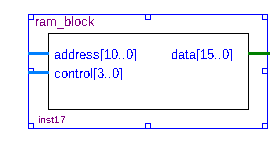
\includegraphics[scale=0.8]{ramb}
    \caption{Блок памяти}
\end{figure}

Блок ram\_block включает в себя синхронные ram и rom, переключение между блоками осуществляется на основе старшего бита адреса.
Временные диаграммы чтения и записи ОЗУ представлены на рисунках 2.1 и 2.2.

Содержимое ROM памяти включает в себя коды команд, записанные последовательно в том порядке, в котором выполняется программа.
Память команд хранится в файле rom.hex.

Блок `ram\_block` содержит 2 входа:
\begin{itemize}
    \item address[10..0] -- адрес ячейки для чтения/записи
    \item control[1..0] -- тактирующий импульс и сигнал режима чтение/запись
\end{itemize}
Двунаправленный вход data[15..0] служит для подключения шины данных.

Содержимое RAM памяти представляет собой данные, которыми оперирует процессор, и в которые происходит запись результатов работы. Содержимое памяти может быть проинициализировано в файле ram.hex.

Синхронная RAM выдает данные на выход на следующем такте, после указания адреса и установления единичного сигнала на входе outenab.

Сигнал inclock на выходах RAM и ROM устанавливается по спаду тактирующего сигнала, outclock -- по фронту.

\subsection{Устройство управления}
Устройство управления устанвливает сигналы, разрешающие работу определенных блоков.
Данный блок представлен в файле 'cu.bdf'.

На вход подается единственный сигнал -- clk. Он служит для тактирования УУ.

\begin{figure}[ht]{\textwidth}
\centering
    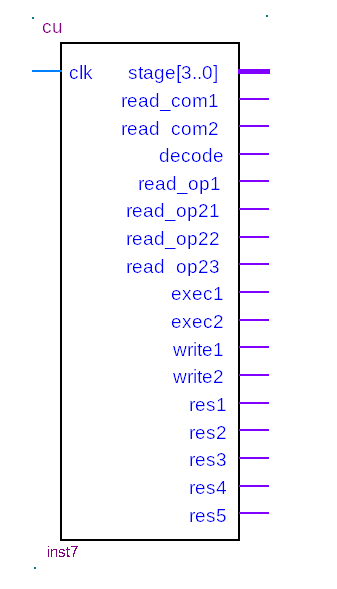
\includegraphics[scale=0.8]{cub}
    \caption{Блок управления}
\end{figure}

Выходы:
\begin{itemize}
    \item stage[3..0] -- отладочный сигнал для наглядного просмотра текущей стадии выполнения команды
    \item read\_com1 -- считывние первого слова команды
    \item read\_com2 -- считывние второго слова команды
    \item decode -- этап декодирования команды
    \item read\_op1 -- чтение первого операнда
    \item read\_op21 -- начало чтения второго операнда
    \item read\_op22 -- запрос в память при косвенной адресации
    \item read\_op23 -- сохранение операнда, полученного из памяти, при косвенной адресации
    \item execute1 -- первый такт операций над операндами
    \item execute2 -- второй такт операций над операндами
    \item write1 -- начало записи результата
    \item write2 -- конец записи результата
    \item res1 - res5 -- резервные выходы
\end{itemize}

\subsection{Блок выборки инструкций}
Данный блок осуществляет выборку инструкций, а также их декодирование.
Блок включает в себя 2 регистра для хранения слов команд, счетчик инструкций.
Схему блока можно найти в файле 'if.bdf'.

\begin{figure}[ht]{\textwidth}
\centering
    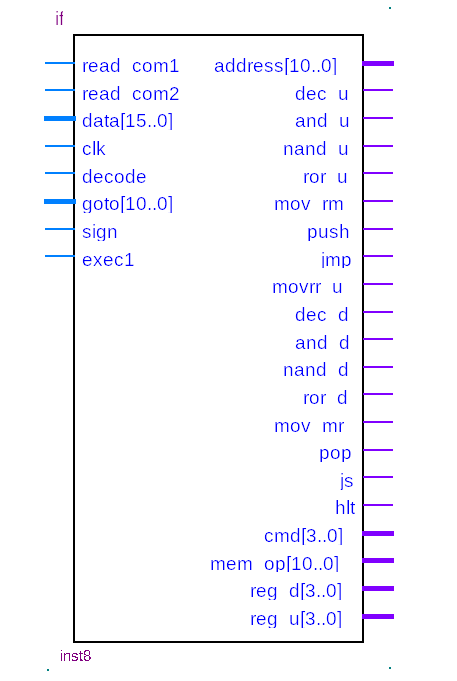
\includegraphics[scale=0.8]{ifc}
    \caption{Блок выборки инструкций}
\end{figure}

Входные сигналы:
\begin{itemize}
    \item clk -- тактирующий сигнал
    \item read\_com1 -- чтение первого слова из памяти
    \item read\_com2 -- чтение второго слова из памяти
    \item decode -- декодирование команды
    \item sign -- флаг знака, служит для операции перехода js
    \item exec1 -- в комбинации с активными сигналами jmp или js и sign приводит к переходу по адресу goto[10..0]
    \item goto[10..0] -- адрес перехода
\end{itemize}
Выходные сигналы:
\begin{itemize}
    \item dec\_d -- декремент. Прямая регистровая адресация
    \item and\_d -- поразрядное И. Прямая регистровая адресация
    \item nand\_d -- поразрядое И-НЕ. Прямая регистровая адресация
    \item ror\_d -- циклический сдвиг вправоИ. Прямая регистровая адресация
    \item dec\_u, and\_u, nand\_u, ror\_u -- аналогичны предыдущим. Косвенная регистровая адресация.
    \item jmp -- безусловный переход
    \item js -- перход при старшем бите равным нулю
    \item hlt -- сигнал выключения микро-ЭВМ
    \item push -- занесение регистра в стек
    \item pop -- чтение регистра из стека
    \item mov\_mr -- пересылка операнда из регистра в память
    \item mov\_rm -- пересылка памяти -> регистр
    \item mov\_rr -- пересылка память -> регистр. Косвенная регистровая адресация
    \item cmd[3..0] -- КОП
    \item mem\_op[10..0] -- адрес операнда, хранящегося в памяти
    \item reg\_d[3..0] -- адрес регистра. Прямая регистровая адресация
    \item reg\_u[3..0] -- адрес регистра. Косвенная регистровая адресация
\end{itemize}

\subsection{Блок выборки операндов}
Осуществляет загрузку операндов из памяти, используя соответсвующую команде адресацию. Блок представлен в файле 'op\_f.bdf'.

\begin{figure}[ht]{\textwidth}
\centering
    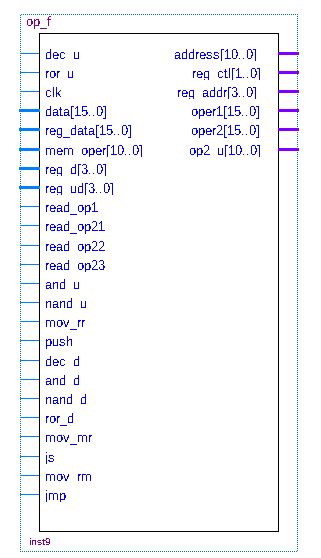
\includegraphics[scale=0.8]{opfb}
    \caption{Блок выборки операндов}
\end{figure}

Входы:
\begin{itemize}
    \item все выходы с предыдущего блока, за исключением hlt, cmd[3..0]
    \item clk -- синхросигнал
    \item reg\_op1 - reg\_op23 -- предоставление процессорного времени
    \item reg\_data[15..0] -- данные из РОН
    \item data[15..0] -- данные из RAM
\end{itemize}
Выходы:
\begin{itemize}
    \item address[10..0] -- адрес для чтения из RAM
    \item reg\_addr[3..0] -- адрес регистра
    \item op1[15..0] -- первый операнд
    \item op2[15..0] -- второй операнд
    \item reg\_ctl[1..0] -- управляющие РОН сигналы
    \item op2\_u[10..0] -- адрес ячейки памяти, при косвенной регистровой адресации
\end{itemize}

\subsection{АЛУ}
Блок АЛУ выполняет арифметические и логические операции, работает со стеком. Если операнды не нуждаются в обработке(например при командах пересылки), АЛУ отправляет их сразу на выход. Также АЛУ содержит регистр, хранящий знак последних выходных данных с АЛУ.

\begin{figure}[ht]{\textwidth}
\centering
    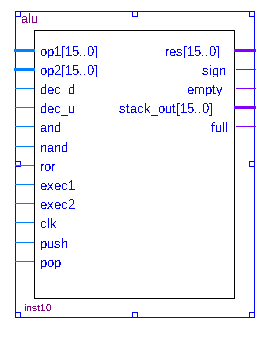
\includegraphics[scale=0.8]{alub}
    \caption{АЛУ}
\end{figure}

Входы:
\begin{itemize}
    \item dec\_d, dec\_u, and, nand, ror, push, pop -- определяют, исполняется ли данная команда сейчас
    \item clk -- синхросигнал
    \item exec1, exec2 -- предоставление процессорного времени
    \item op1[15..0] -- первый операнд
    \item op2[15..0] -- второй операнд
\end{itemize}
Выходы:
\begin{itemize}
    \item res[15..0] -- выходной операнд
    \item stack\_out[15..0] -- данные, выходящие со стека
    \item sign -- флаг установки старшего бита в 1
    \item empty -- стек пуст
    \item full -- стек полон
\end{itemize}

\subsection{Блок сохранения результата}

\begin{figure}[ht]{\textwidth}
\centering
    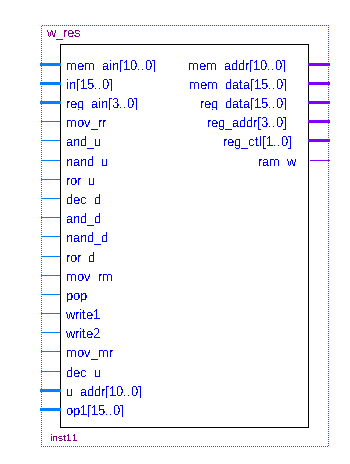
\includegraphics[scale=0.8]{wbc}
    \caption{Блок сохранения результата}
\end{figure}
Входы:
\begin{itemize}
    \item mem\_ain[10..0] -- адрес для записи данных при прямой адресации
    \item in[15..0] -- операнд для записи
    \item u\_addr[10..0] -- адрес для записи операнда при косвенной регистровой адресации
    \item op1[15..0] -- вход для операнда команды dec
    \item write1, write2 -- сигналы разрешения работы
\end{itemize}
Выходы:
\begin{itemize}
    \item ram\_w -- сигнал переключения RAM в режим записи
    \item reg\_ctl[1..0] -- управляющие сигналы РОН
    \item reg\_addr[3..0] -- адрес РОН
    \item reg\_data[15..0] -- данные для записи в РОН
    \item mem\_data[15..0] -- данные для ОЗУ
    \item mem\_addr[10..0] -- адрес памяти для записи операнда
\end{itemize}
Остальные входы -- входы работы соответствующих команд
Блок осуществляет запись операнда в ОЗУ или РОН в зависимости от адресации команды.

\subsection{Блок РОН}
\begin{figure}[ht]{\textwidth}
\centering
    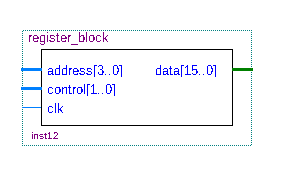
\includegraphics[scale=0.8]{regb}
    \caption{Блок РОН}
\end{figure}

Входы:
\begin{itemize}
    \item address[3..0] -- адрес регистра
    \item control[1..0] -- управляющий вход
    \item clk -- синхросигнал
\end{itemize}
Двунапраленные порты:
\begin{itemize}
    \item data[15..0] -- данные
\end{itemize}

Блок РОН содержит 10 шестнадцатиразрядных регистров общего назначения. Регистры могут хранить как данные, так и адреса ячеек памяти.

\subsection{Стек}
Содержит 11 шестнадцатиразрядных регистров. Позволяет работать с регистрами по принципу FIFO. На схеме блок имеет название 'Stack'.

\begin{figure}[ht]{\textwidth}
\centering
    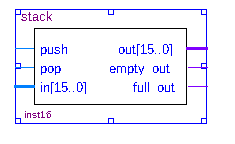
\includegraphics[scale=0.8]{stackb}
    \caption{Стек}
\end{figure}

Входы:
\begin{itemize}
    \item push -- запись регистра в стек
    \item pop -- освобождение регистра из стека
    \item in[15..0] -- входной регистр
\end{itemize}
Выходы:
\begin{itemize}
    \item out[15..0] -- выходной регистр
    \item empty -- стек пуст
    \item full -- стек полон
\end{itemize}
Стек растет вверх, указатель стека указывает на следующую свободную ячейку.
При включении сигнала full -- запись в стек блокируется, при активном сигнале empty -- отсутствует запись операнда команды pop на шаге сохранения операндов.

